% !TeX root = ../../../book.tex

\subsection{等价类}

\subsubsection*{定义}

假设我们在集合 $A$ 上定义了一个等价关系 $R$。我们之所以做出以下定义,是因为在前几段中已经有所提示。这三个性质 --- 自反性、对称性和传递性 --- 共同作用,将集合 $A$ 划分为若干个标准\emph{划分}。任何相互关联的元素都会形成一个``封闭组织''或``簇'',因此我们可以将这些``组织''中的任意元素作为代表,而不必全部列出。这些``组织''被称为\emph{等价类},以下定义将进一步探讨这一概念。

\begin{definition}
    设 $R$ 为集合 $A$ 上的等价关系,并设 $x \in A$。(关系 $R$ 下的)$x$ 的\dotuline{等价类}是与 $x$ 相关的所有元素的集合,写做 $[x]_R$。即
    \[[x]_R = \{y \in A \mid (x,y) \in R\}\]
\end{definition}

\subsubsection*{引言与示例}

这个定义的核心思想是,等价类可以让我们根据关系 $R$ 将集合 $A$ \textbf{划分}为若干个标准集合。回顾第 \ref{ch:chapter03} 章中的定义 \ref{def:definition3.6.9},可以看到我们是如何定义集合\textbf{划分}的。(实际上,可以再看一下定义 \ref{def:definition4.5.11},了解我们如何用逻辑符号重新表述这个定义。)现在,只需记住,划分是非空集合的集合,这些集合彼此互不相交,并且它们的并集构成了整个要讨论的集合。\\

\begin{example}
    让我们回到本节一开始的例子。我们在实数集 $\mathbb{R}$ 上定义了一个关系 $R$,如下所示:
    \[\forall x, y \in \mathbb{R} \centerdot (x, y) \in \mathbb{R} \iff \lfloor x \rfloor = \lfloor y \rfloor\]
    现在,利用这个定义来思考一个特定的等价类。具体来说,我们来看
    \[[0]_R = \{y \in \mathbb{R} \mid (0, y) \in \mathbb{R}\} = \{\in \mathbb{R} \mid \lfloor 0 \rfloor = \lfloor y \rfloor\} = \{y \in \mathbb{R} \mid \lfloor y \rfloor = 0\} = \{y \in \mathbb{R} \mid 0 \le y < 1\}\]
    通过上述 $[0]_R$ 的定义、关系 $R$ 的定义,以及对 $\lfloor y \rfloor$ 的理解,我们可以知道\emph{在关系 $R$ 下,$0$ 的等价类}是从 $0$(包含)到 $1$(不包含)这个区间。我们可以用下图表示这个区间:

    \begin{center}
        {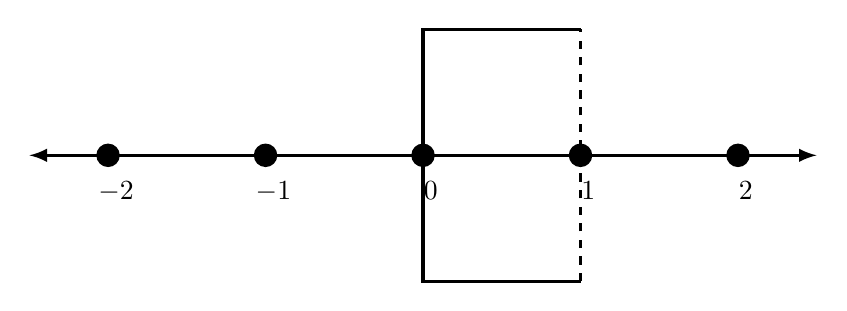
\begin{tikzpicture}[very thick,scale=2]
            \draw[latex-latex] (-2.5,0) -- (2.5,0); 
            \foreach \x in  {-2,-1,0,1,2}
            {
                \node at (\x, 0)[circle,fill,inner sep=3pt]{};
                \draw[shift={(\x+0.05,-0.1)}] node[below] {$\x$};
            }
            \draw[dashed] (1,-0.8) -- (1,0.8);
            \draw (1,0.8) -- (0,0.8) -- (0, -0.8) -- (1, -0.8);
        \end{tikzpicture}}
    \end{center}

    同理,我们可以得到
    \[[1]_R = \{y \in \mathbb{R} \mid (1, y) \in \mathbb{R}\} = \{y \in \mathbb{R} \mid 1 \le y < 2\}\]
    如下图所示:

    \begin{center}
        {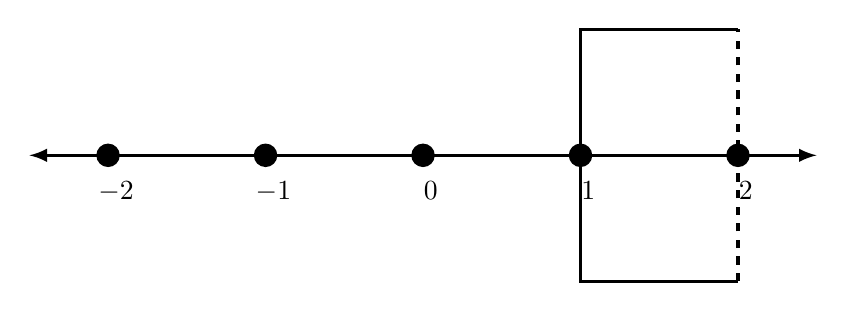
\begin{tikzpicture}[very thick,scale=2]
            \draw[latex-latex] (-2.5,0) -- (2.5,0); 
            \foreach \x in  {-2,-1,0,1,2}
            {
                \node at (\x, 0)[circle,fill,inner sep=3pt]{};
                \draw[shift={(\x+0.05,-0.1)}] node[below] {$\x$};
            }
            \draw[dashed] (2,-0.8) -- (2,0.8);
            \draw (2,0.8) -- (1,0.8) -- (1, -0.8) -- (2, -0.8);
        \end{tikzpicture}}
    \end{center}
\end{example}

请注意,这两个集合是互不相交的,因为第一个集合不包含 $1$,而第二个集合包含 $1$。此外,\emph{每个}实数都\emph{恰好属于一个}这样的区间。例如,我们可以说
\[\pi \in [3]_R, e \in [2]_R, -1.5 \in [-2]_R,\frac{1}{2} \in [0]_R\]
请注意,\emph{等价类}的定义并没有要求我们必须用一个元素来\emph{表示}该类。例如,我们也可以这样说
\[[0]_R = \Big[\frac{1}{2}\Big]_R\]
因为这两个集合是相等的,它们包含相同的元素。任何``向下取整'' 为 $0$ 的实数在 $R$ 下都与 $0$ 相关,因此在 $R$ 下也与 $\frac{1}{2}$ 相关,因为它们的向下取整都是 $0$。

多探索一下这个例子,尝试说服自己,这个划分属性在这里确实有效。在下一部分,我们将在你的帮助下正式证明这一事实的普遍性!由于接下来的讨论会比较抽象,我们建议你多通过实际例子来理解。尝试在另一个集合上定义一个等价关系。它的等价类是什么?你能理解为什么它们会构成一个划分吗?

\subsubsection*{等价类划分集合}

我们已经探讨了等价类\emph{划分}集合的思想,接下来让我们来正式定义这个概念。我们需要先给出一个定义,然后再证明一个定理!这个定理本质上是一个``当且仅当''定理,我们将证明其中一个方向,另一个方向留作练习。

\begin{definition}
    设 $R$ 为集合 $A$ 上的等价关系,关系 $R$ 下等价类的集合记作 $A / R$,即 $A$ \dotuline{模 (modulo)} $R$。也就是说
    \[A / R = \{[x]_R \mid x \in A\}\]
    换种写法是
    \[A / R = \{X \subseteq A \mid \exists x \in A \centerdot X = [x]_R\}\]
\end{definition}

在我们证明重要结果之前,先来看几个例子来理解这些概念。在每个例子中,我们要判断是否存在等价关系,检验等价类,并思考模运算的作用。\\

\begin{example}
    再次考虑定义在实数集 $\mathbb{R}$ 上的关系 $R$ ,其定义为 $(x, y) \in R \iff \lfloor x \rfloor = \lfloor y \rfloor$。我们之前已经讨论过为什么这是一个等价关系,现在让我们来研究一下它的等价类。

    根据定义,任何两个相关的元素都有相同的等价类。例如,$[0]_R = [0.5]_R = [0.999]_R$。同样地,$[3.5]_R = [3.75]_R$ ,以及 $[-\pi]_R = [-4]_R$ ,但 $[\pi]_R = [4]_R$。每个实数 $x \in \mathbb{R}$ 都有一个对应的等价类 $[x]_R$,而模运算的思想是通过只考虑必要的等价类来简化 $R$ 的表示。由于 $[0]_R = [0.5]_R = [0.333]_R$ 等等,我们可以用一个集合 $[0]_R$ 来代表所有这些相同的集合。因此,我们可以表示
    \[\mathbb{R} / R = \{\dots, [-2]_R, [-1]_R, [0]_R, [1]_R, [2]_R, \dots \}\]
    实际上,$\mathbb{R} / R$ 可以看作是整数集 $\mathbb{Z}$。然而,我们通常写作 $\mathbb{R} / R ``='' \mathbb{Z}$ 是因为这种等式并不完全准确。特别是,我们还没有严格推导出实数或整数,仅仅严格定义了自然数 $\mathbb{N}$。在这里,我们只是观察到等价类集合与整数集合之间的某种对应关系。我们可以将一个对应到另一个,反之亦然,但这并不意味着它们在技术上是\emph{相等的}。

    不过没关系!这个例子的主要目的是指出 $\mathbb{R} / R$ 是一个等价类的集合。记住,当我们写下一个集合时,顺序和重复是无关紧要的。也就是说, $\{1, 3, 5, 3, 1\}$ 在集合意义上等于 $\{1, 3, 5\}$。它们具有\emph{相同元素},因此是\emph{相同对象}。在当前的上下文中,我们不需要在集合  $\mathbb{R} / R$ 中同时包含 $[0]_R$ 和 $[0.5]_R$,因为它们是同一个对象;在我们的元素列表中重复该对象没有任何意义。

    通常,我们会关注识别等价类的形式并提供一些定性的描述。特别是,我们会经常思考在 $A/R$ 中有多少个等价类。我们还会关注这些类的大小。它们都是一样大的吗?是不是有些类只有几个元素,而有些类则是无穷大的?为什么会这样?这些类元素的``描述''是否大致相同?

    在这个特定的例子中,我们发现 $\mathbb{R} / R$ 中的所有等价类在形式上非常相似。有无限多个等价类 --- 每个整数 $\mathbb{Z}$ 的元素都是一个 --- 它们都是无穷大的,包含一个实数区间。此外,所有这些类的形式都是对于某个 $z \in \mathbb{Z}, [z]_R = \{y \in \mathbb{R} \mid z \le y < z + 1\}$。从这个意义上说,这些等价类都是\emph{性质相似}的。
\end{example}

\begin{example}
    在所有人的集合 $S$ 上定义关系 $B$ 为 $(x, y) \in B \iff x \;\text{和}\; y \;\text{同一个月出生}$。那么 $(\text{欧拉}, \text{庞加莱}) \in B$ 且 $(\text{Paul Erdös}, \text{Emmy Noether}) \in B$。为什么这是等价关系?任何人都与自己相同月份出生(自反性)。如果两个人同一月份出生,那么他们的出生月份是相同的(对称性)。如果 $x$ 和 $y$ 同一月份出生,$y$ 和 $z$ 同一月份出生,那么 $x$ 和 $z$ 也是同一月份出生(传递性)。

    (注意:通常由``有相同的……''或``是相同的……''定义的关系是等价关系。)

    在这个关系下,等价类对应的是月份。因为我们用出生月份来区分人群,一个等价类就是一组同月出生的人。例如,Paul Erdös 和 Emmy Noether 都是三月出生,所以我们可以说 $\text{Emmy Noether} \in [\text{Paul Erdös}]_B$ 这个等价类。这个等价类\emph{对应于}三月,但请注意,它是根据集合 $S$ (所有人)中的特定元素定义的。

    如果我们定义 $M$ 为所有三月出生的人的集合,那么我们可以说 $M = [\text{Paul Erdös}]_B$。综合这些观察,我们可以得出结论:按出生月份划分人的集合,记为 $S/B$,由 $12$ 个集合组成,每个集合对应一个不同月份,并包含所有在那个月份出生的人。
\end{example}

\begin{example}
    考虑所有有序实数对的集合 $\mathbb{R} \times \mathbb{R}$。我们通过定义两个对何时\emph{相关}来定义 $\mathbb{R} \times \mathbb{R}$ 上的关系 $R$。具体来说,我们定义
    \[\big((x, y),(u, v)\big) \in R \iff x = u\]
    也就是说,当平面上的两点第一个坐标相同时,它们在关系 $R$ 下是相关的。想想为什么这是一个等价关系?从几何上讲,这个关系只关心一个点所在的垂直于 $y$ 轴的直线。理解这一点后,你可以很容易地``看出''并解释为什么 $R$ 是一个等价关系,而严格证明这一点只需要多写一些内容和符号。(试试看!)

    这也使我们能够轻松描述和可视化这个关系下的等价类。所有在同一垂线上的点都属于同一个等价类,我们可以通过查看这些垂线与水平轴的交点来索引这些类。例如,$(1, 3) \in [(1, 0)]_R$,因为点 $(1, 3)$ 和 $(1, 0)$ 位于同一条垂线上。我们可以用这种方式表示\emph{每一个}等价类:$[(x, 0)]_R$,其中 $x \in \mathbb{R}$。
\end{example}

\begin{center}
    {\begin{tikzpicture}[very thick,scale=2]
        \draw[latex-latex] (-1.5,0) -- (2.5,0); 
        \draw[latex-latex] (0,-1.5) -- (0,3.5); 
        \foreach \x in  {1,2}
        {
            \node at (\x, 0)[circle,fill,inner sep=3pt]{};
            \draw[shift={(\x+0.25,-0.1)}] node[below] {$(\x, 0)$};
        }
        \foreach \y in  {1,2,3}
        {
            \node at (0, \y)[circle,fill,inner sep=3pt]{};
            \draw[shift={(-0.15, \y)}] node[left] {$(0, \y)$};
        }
        \draw[dashed] (1,-1.5) -- (1,3.5);
        \node at (1, 3)[circle,fill,inner sep=3pt]{};
        \draw[shift={(1.15, 3)}] node[right] {$(1, 3)$};
        \draw[shift={(1.15, 1.5)}] node[right] {$[(1,0)]_R = \{(1, y)\}$};
    \end{tikzpicture}}
\end{center}

因此,在某种意义上,等价类的集合 $(\mathbb{R} \times \mathbb{R})/R$ 与实数轴 $\mathbb{R}$ 是``等同的''!通过忽略第二个坐标,我们可以将平面上的所有点压缩到水平轴上。从数学上讲,有一种方法可以更精确地表达这个想法,但在此我们无法正式讨论。简单来说,$\mathbb{R} \times \mathbb{R}$ 上的这个关系产生的等价类由 $\mathbb{R}$ 表示,这其中存在一些有趣的现象。

这里有另一个 $\mathbb{R} \times \mathbb{R}$ 上的关系。定义 $S$ 为
\[\big((x, y),(u, v)\big) \in S \iff \sqrt{x^2+y^2} = \sqrt{u^2+v^2}\]
回想一下基本的几何和代数知识,你可能会发现表达式 $\sqrt{x^2 + y^2}$ 描述的是点 $(x, y)$ 到原点 $(0, 0)$ 的距离。(在数学中,我们称这种表达式为\emph{度量 (metric)}。)因此,这个关系表明,当两点到原点的距离相同时,它们是等价的。从视觉上来看,这解释了为什么 $S$ 是一个等价关系,并且展示了等价类是以原点为中心的圆。因此,我们可以通过这些圆的一个显著特征 --- 它们的\emph{半径} $r \ge 0$,来描述集合 $(\mathbb{R} \times \mathbb{R})/S$ 的元素。因此,在 $S$ 下的等价类集合与非负实数集合是``等同的''!

\begin{center}
    {\begin{tikzpicture}[very thick,scale=2]
        \draw[latex-latex] (-3,0) -- (3,0); 
        \draw[latex-latex] (0,-3) -- (0,3); 
        \foreach \x in  {-2,-1,0,1,2}
        {
            \node at (\x, 0)[circle,fill,inner sep=3pt]{};
            \node at (0, \x)[circle,fill,inner sep=3pt]{};
        }
        \draw[dashed] (0,0) circle (1);
        \draw[dashed] (0,0) circle (2);
        \draw[shift={(0.8, -0.7)}] node[right] {$[(1,0)]_S$};
        \draw[shift={(0.8, -0.9)}] node[right] {$r=1$};
        \draw[shift={(1.7, 1.5)}] node[right] {$[(2,0)]_S$};
        \draw[shift={(1.7, 1.3)}] node[right] {$r=2$};
    \end{tikzpicture}}
\end{center}

这听起来有点奇怪,对吧?我们从一个二维集合开始,关联成对的点,并整理出等价类,结果得到了一个一维集合。(注意:我们这里还没有正式的方法来定义\emph{维度},但你应该能理解我们的意思。)回顾一下上面在 $\mathbb{R}^2$ 上定义的关系 $R$。如果我们只在 $\mathbb{R}^2$ 的``右半部分''定义这个关系,也就是所有第一个坐标非负的点,那么等价类的集合也会和非负实数集合``相同''。从哪个角度看,这个集合和 $(\mathbb{R} \times \mathbb{R})/S$ 是``相同''的呢?这个问题合理吗?我们该如何\emph{证明}此说法?这些都是非常有趣的问题,我们鼓励你思考一下这些问题!

不要过于纠结于这些概念和问题。关键在于:等价类的集合构成底层集合的\textbf{划分}。

现在我们已经看过了若干例子,接下来我们来陈述(并证明!)一些关于等价关系的重要结论。主要是,这些定理说明了我们一直暗示的观点,即等价关系会将集合划分成相应的等价类。不过,令人惊讶的是,我们还有一个有趣的结论:给定任意一个划分,我们可以为其定义一个等价关系!

\begin{theorem}\label{theorem6.4.10}
    设 $R$ 为集合 $A$ 上的等价关系。则属于 $A/R$ 的集合构成 $A$ 的划分。也就是说,它们是非空的,互不相交的,它们的并集是 $A$。
\end{theorem}

\begin{proof}
    见习题 \ref{exc:exercises6.7.13}
\end{proof}

我们将在本章末尾的习题 \ref{exc:exercises6.7.13} 中带你完成这个结论的证明。我们之前研究的例子应该可以帮助你直观地理解为什么这个定理是正确的,而通过详细地推导证明过程,你将对其背后的数学严谨性有一个扎实的理解。

\subsubsection*{划分产生等价关系}

现在,我们来看一个类似且重要的结论,这是前一个定理的逆命题。为了更好地理解这个定理,我们先看一个例子,这个例子还将为我们提供定理证明的概要。\\

\begin{example}
    考虑集合 $S=[6]$。定义集合
    \[\mathcal{F} = \{ \{1, 4\}, \{2, 3, 5\} , \{6\} \}\]
    注意,$\mathcal{F}$ 是 $S$ 的一个划分,因为这些集合是互不相交的,非空的,且它们的并集是 $S$。如果有一种等价关系 $R$,使得我们在考虑 $S/R$ 时得到这些集合,那不是很好吗?事实上,确实存在这样的关系!尽管我们可能无法像之前那样,以一种优雅的方式定义它们,例如通常的``$(x, y) \in R \iff x \;\text{和}\; y \;\text{具有某种共同属性}$''。不过,既然我们已经有了划分,就可以用它来定义关系。具体来说,划分集合就是等价类。划分本身建立了等价类的结构,我们只需通过 $(x, y) \in R \iff x \;\text{和}\; y \;\text{属于同一个划分集合}$ 来定义等价关系 $R$。

    在本例中,我们可以定义 $S_1 = \{1, 4\} , S_2 = \{2, 3, 5\} , S_3 = \{6\}$,则我们可以定义 $R$
    \[(x, y) \in R \iff \exists i \in [3] \centerdot (x \in S_i \land y \in S_i)\]
\end{example}

想一想为什么这种方法有效。你能理解为什么这是一个等价关系吗?你知道等价类是什么吗?

现在我们准备陈述并证明这个定理。

\begin{theorem}\label{theorem6.4.12}
    设 $S$ 为集合,并设 $\mathcal{F}$ 为集合 $S$ 的划分。则存在等价关系 $R$ 使得 $S/R=\mathcal{F}$。
\end{theorem}

正如我们之前提到的,这个结果完全依赖于一个事实:划分是一组集合,这些集合正是我们要定义的等价类。我们只需要证明``$x$ 和 $y$ 相关当且仅当 $x$ 和 $y$ 属于同一个划分集合''这个关系是一个等价关系。这并不难!在阅读我们的证明之前,试着自己勾画一下证明的细节吧!

\begin{proof}
    设 $\mathcal{F}$ 为集合 $S$ 的划分。这意味着我们有一个索引集 $I$,且
    \[\mathcal{F} = {S_i \mid i \in I}\]
    其中集合 $S_i$ 满足 $S_i \subseteq S$ 且 $S_i \ne \varnothing$ 且
    \[\bigcup_{i \in I} S_i = S \quad \text{且} \quad \forall i, j \in I \centerdot i \ne j \implies S_i \cap S_j = \varnothing\]
    定义 $S$ 上的关系 $R$ 为
    \[(x, y) \in R \iff \exists i \in I \centerdot (x \in S_i \land y \in S_i)\]
    我们要证明 $R$ 是等价关系。

    \begin{itemize}
        \item 设 $x \in S$ 是任意固定的。由于 $S_i$ 的集合覆盖 $S$,因此我们知道 $\exists i \in I \centerdot x \in S_i$。给定这样的 $i$,则必然有 $x \in S_i$ 且 $x \in S_i$,所以 $(x,x) \in R$。因此 $R$ 具有自反性。
        \item 设 $x, y \in S$ 是任意固定的。假设 $(x, y) \in R$。这意味着 $\exists i \in I \centerdot (x \in S_i \land y \in S_i)$。给定这样的 $i$,则必然有 $y \in S_i \land x \in S_i$,所以 $(y,x) \in R$。因此 $R$ 具有对称性。
        \item 设 $x, y, z \in S$ 是任意固定的。假设 $(x, y) \in R$ 且 $(y, z) \in R$。这意味着 $\exists i \in I \centerdot (x \in S_i \land y \in S_i)$ 且 $\exists j \in I \centerdot (y \in S_j \land z \in S_j)$。给定这样的 $i,j$,注意 $y \in S_i \land y \in S_j$,而对于任意不同的 $i,j, S_i \cap S_j = \varnothing$,因此 $i=j$(否则会出现 $y \in \varnothing$,而这是不可能的!)由于 $x \in S_i, y \in S_i, z \in S_i$,所以 $(x,z) \in R$。因此 $R$ 具有传递性。
    \end{itemize}
    由于上面三个性质成立,所以 $R$ 是一个等价关系!

    $S/R$ 的等价类写做 $[x]_R$,其中 $x \in S$。因为 $\mathcal{F}$ 是 $A$ 的分割,对于某个 $i, x \in S_i$,所以对于某个 $i, [x]_R = S_i$。因此所有等级类等于某集合 $S_i$。

    类似地,任意集合 $S_i \ne \varnothing$,所以 $\exists x \in S_i$,因此存在对应的等价类 $S_i=[x]_R$。因此,每个等价类都是形如 $S_i$ 的集合,反之亦然。
\end{proof}

这表明,任何划分都可以很好地对应一个等价关系及其等价类!
